%%%%%%%%%%%%%%%%%%%%%%%%%%%%%%%%%%%%%%%%%
% University Assignment Title Page 
% LaTeX Template
% Version 1.0 (27/12/12)
%
% This template has been downloaded from:
% http://www.LaTeXTemplates.com
%
% Original author:
% WikiBooks (http://en.wikibooks.org/wiki/LaTeX/Title_Creation)
%
% License:
% CC BY-NC-SA 3.0 (http://creativecommons.org/licenses/by-nc-sa/3.0/)
% 
% Modified for COSC480/490 by:
% Lech Szymanski (8/3/18)

\documentclass[12pt]{article}
\usepackage[draft]{cosc4x0style}
\usepackage[ruled, linesnumbered,lined]{algorithm2e}
\usepackage{amsmath}
\usepackage{amssymb}
\usepackage{amsthm}
\usepackage{breakcites}
\usepackage{color}
\usepackage{caption}
\usepackage[linguistics]{forest}
\usepackage{longtable}
\usepackage{marginnote}
\usepackage{todonotes}
\usepackage{subcaption}
\usepackage{rotating}
\usepackage{url}

% Custom theorem environment stuff %
% Gets rid of italics
% \theoremstyle{definition}
\newtheoremstyle{grammarstyle}% name
  {10pt}%Space above
  {10pt}%Space below
  {\normalfont}%Body font
  {\parindent}%Indent amount
  {\bfseries}% Theorem head font
  {:}%Punctuation after theorem head
  {\parindent}%Space after theorem head 2
  {}%Theorem head spec (can be left empty, meaning ‘normal’)
\theoremstyle{grammarstyle}

\newtheorem{gram}{Grammar}
% \numberwithin{align}{gram}

% Replace the trailing period with a colon
% \usepackage{xpatch}
% \makeatletter
% \xpatchcmd{\@thm}{\thm@headpunct{.}}{\thm@headpunct{}}{}{}
% \makeatother

% Get rid of parantheses around optional argument
\makeatletter
\def\thmhead@plain#1#2#3{%
  \thmname{#1}\thmnumber{\@ifnotempty{#1}{ }\@upn{#2}}%
  \thmnote{ {\the\thm@notefont#3}}}
\let\thmhead\thmhead@plain
\makeatother

% Code listings styles %
\usepackage{listings}
\usepackage{xcolor}
 
\definecolor{codegreen}{rgb}{0,0.6,0}
\definecolor{codegray}{rgb}{0.5,0.5,0.5}
\definecolor{codepurple}{rgb}{0.58,0,0.82}
 
\lstdefinestyle{mystyle}{
    commentstyle=\color{codegreen},
    keywordstyle=\color{magenta},
    numberstyle=\tiny\color{codegray},
    stringstyle=\color{codepurple},
    basicstyle=\ttfamily\footnotesize,
    breakatwhitespace=false,         
    breaklines=true,                 
    captionpos=b,                    
    keepspaces=true,                 
    numbers=left,                    
    numbersep=5pt,                  
    showspaces=false,                
    showstringspaces=false,
    showtabs=false,                  
    tabsize=2
}
 
\lstset{style=mystyle}

\newcommand{\keyword}[1]{%
    \textbf{#1}%
    % Add keyword to the margin
    % \todo[color=none, linecolor=none]{#1}%
}

\usepackage[round]{natbib}   % omit 'round' option if you prefer square brackets
\bibliographystyle{plainnat}
% \bibliographystyle{apalike}
% \usepackage[usenames,dvipsnames,svgnames,table]{xcolor}

% To compile the final version of the report (which will remove all the todo content)
%\usepackage{cosc4x0style}

% Specify project code 480 or 490
\papercode{480}

% Your project title
\title{Quantifying Conceptual Density in Text}

% Your name
\author{Anthony \textsc{Dickson}}
\studentid{3348967}

% Names of your supervisors, separated by line break '\\'
\supervisors{
  Anthony \textsc{Robins} \\
  Alistair \textsc{Knott}
}

% Date, change the \today to a set date if you want to be precise
\reportdate{\today}

\begin{document}
\maketitle

\begin{abstract}
    It has been claimed that programming languages form a domain of \textit{tightly integrated} concepts and that these tightly integrated concepts are difficult to describe or understand independently of other concepts. This tightly integrated nature of concepts in programming languages is thought to lead to the high rate of both fail and high grades observed in introductory programming courses across many institutions. This notion of the degree to which concepts are integrated in a domain is referred to as \textbf{conceptual density}. In this project we are interested in conceptual density in general, not just in the context of programming languages. In this report a definition of conceptual density and a graph-based method for quantifying conceptual density in well-structured expository text documents, such as educational textbooks, are explored. 
    % Talk about why measuring conceptual density would be useful?
\end{abstract}

% \tableofcontents
% \clearpage

\section{Introduction}
It is thought that the unusually high rate of fail and high grades observed in introductory programming courses is possibly due to concepts in programming languages being unusually tightly integrated \citep{robins2010learning}. A tightly integrated concept is a concept that is difficult to describe independently of other concepts. Tightly integrated concepts are said to magnify the effects of learning edge momentum and lead to the polarised outcomes observed in introductory programming courses. This report is interested in conceptual density, an idea related to the degree to which concepts in a given domain are integrated.  

The idea of conceptual density affecting learning difficulty is not unique to the aforementioned work. It appears in the literature on cognitive load theory, in a perhaps slightly different form, as the ``element interactivity effect'', which says that the number of interacting elements in a task is the main contributor to cognitive load - a measure of mental exertion required to perform a given task \citep{sweller1994cognitive}. Cognitive load theory provides an explanation of aspects of learning difficulty and can be used to guide education and instructional design.

To the best of my knowledge there exists no objective measure in the current literature of the element interactivity effect, or the notion of conceptual density. Element interactivity appears to be estimated manually and it depends greatly on the knowledge of the learner \citep{chandler1996cognitive}, and as such remains subjective. In \citep{robins2010learning} the notion of concepts being tightly integrated stems from the observation that educators typically fail to reach a consensus on how to structure introductory programming courses (this is supposedly not the case in many other disciplines).  While no measure of conceptual density was clearly defined in that work, some possible ways to do so were proposed.

In this report,  I follow up on the notion of conceptual density and set out to elaborate on its definition and develop an objective measure of conceptual density in the context of well-structured expository text documents (e.g. textbooks, scientific papers). For measuring conceptual density I explore one of the methods mentioned in \citep{robins2010learning} - analysing a mind-map like graph structure. Whereas in the original work, this approach was suggested as a characterisation of introductory programming course material that is to be generated by experts, in this report I aim to build up and analyse mind-map like graph structures through the use of natural language processing methods and graph analysis techniques, removing the need for an expert to manually assess conceptual density for a given document.

The rest of this report is structured as follows: Section \ref{sec:background} covers the theoretical background of conceptual density; Section \ref{sec:conceptual_density_in_text} defines what is considered as a concept in text and other text features that relate to conceptual density; Section \ref{sec:building_a_mind-map} describes the parsing algorithm used for building a mind-map like graph structure and how a numerical score of conceptual density can be derived from a graph structure; Section \ref{sec:related_work} discusses related work and what distinguishes the work in this project from the related work; and Section \ref{sec:future_work} discusses the work-to-date and future work.

\section{Background} \label{sec:background}
\subsection{Learning Edge Momentum}
Learning edge momentum was proposed as an explanation for the unusually high rate of both fail and high grades in introductory computer science courses \citep{robins2010learning}. The hypothesis builds upon the idea that we learn at the edges of what we know - it is easy to learn things that build upon pre-existing knowledge. The core of the hypothesis is that learning outcomes are self-reinforcing: successful learning  tends to make learning closely related concepts easier, and unsuccessful learning tends to make learning closely related concepts more difficult. It is also said that concepts in programming languages tend to be tightly integrated and that these tightly integrated concepts are difficult to describe or understand independently of each other. This means that learning a new concept is greatly dependent on understanding the prerequisite concepts. And because of this the effects of learning edge momentum in introductory programming courses are particularly pronounced, leading to the polarised distribution of grades. 

Conceptual density is mentioned in this paper as a possible metric for providing more concrete evidence to educators on how to structure an introductory programming course. Two methods are suggested for measuring the degree to which concepts in a domain are integrated. One method is to look at the proximity of key concept terms and see if there are areas where many concepts are mentioned close together. The other method is to generate a mind-map like graph structure A Here we represent the domain of concepts as a graph structure, where the concepts present in the material are represented with a node in the graph and edges between nodes represent a connection between concepts. This follows the main ideas behind semantic networks and knowledge graphs \citep{sowa1987semantic, zhang2002knowledge, koncel2019text}, an area of research concerning knowledge representation using graphs. This idea of a mind map of concepts forms the basis for the work in this project.

\subsection{Cognitive Load Theory}
Cognitive load theory provides a framework about learning difficulty and instructional design \citep{sweller1994cognitive}. In CLT (cognitive load theory) the main task of the brain is characterised as information processing, and each person has a certain amount of working memory to process information. Performing tasks requires an amount of mental exertion and concentration, called cognitive load. When the amount of cognitive load exceeds the capacity of an individual's working memory, performing the given task becomes much more difficult. 

If we are to explain this by analogy, the idea of working memory is similar in some ways to computer RAM and running out of working memory is akin to what happens when a computer runs out of RAM. When a computer runs out of RAM, it starts thrashing and all of the programs will become very slow and take many times longer to run compared to when there is enough RAM. By reducing the number of programs that are running we can reduce the memory usage and prevent the computer from thrashing. Similarly, under CLT we can reduce cognitive load by reducing the number of things that must be considered simultaneously to perform a given task in order to make it easier to perform that task. 

The main contributor to the difficulty of a task is number of things that must be considered simultaneously and the degree to which they interact. In CLT this idea is captured by the \keyword{element interactivity effect} \citep{sweller2011element}. The cognitive load imposed by element interactivity is said to be intrinsic to the material itself (\keyword{intrinsic cognitive load}), meaning that no matter how you present the material there will be a minimum level of difficulty.

How we present material can affect how difficult it is understand it. For example, consider trying to teach beginner programmers what all of the keywords mean in a Java program that simply prints a message to the screen (see Figure \ref{fig:java_hello_world}) and what each part of the code does. This would likely be too much to learn at once. Here there are many interacting elements (e.g. access modifiers, classes, types, functions, function arguments, comments, member fields, member functions, function calls, string literals) just in this simple program. Compare this to simply pointing out the line that prints the message and the fact that anything between the quotation marks is printed to the terminal window. This approach is much easier to understand since there are fewer things that must be considered. Changing how the material is presented has the effect of increasing or reducing \keyword{extraneous cognitive load}, a type of cognitive load that is not intrinsic to the material itself but dependent on how the material is presented. 

\begin{figure}
    \centering
     \lstset{xleftmargin=20pt}
    \lstinputlisting[language=Java]{docs/HelloWorld.java}
    \caption{Java hello world example}
    \label{fig:java_hello_world}
\end{figure}

Following on with the example, the details of the ``Hello, world!'' program could be taught more easily once the learner has learned the fundamentals and acquired a basic intuition for programming. It is theorised that this is because as complex ideas and tasks are learned, we learn more compact representation of these. These compact representations are often referred to as a \keyword{schema}; a schema is essentially a single unit of knowledge representing a concept or task \citep{axelrod1973schema, abelson1981psychological, bartlett1995remembering}. By acquiring a schema, a task with many interacting elements can be reduced to a task with a few, or even a single, element. And under the element interactivity effect fewer interacting elements means less overall cognitive load. This idea of learned knowledge reducing the complexity of a task or idea is captured by \keyword{germane cognitive load}. Essentially, germane load is a type of cognitive load incurred by accessing schema. The amount of cognitive load incurred by this type of cognitive load is less than other types due to the use of schemas and their effect of reducing a complex idea/task down to a more compact representation.

To summarise CLT in a rather simplified manner, an individual has a limited amount of working memory to perform tasks and if the amount of cognitive load exceeds the capacity of this working memory, performing the given task becomes much more difficult. There is one major effect and three types of cognitive load that we are interested in: the element interactivity effect which is the main contributor to intrinsic load and overall cognitive load; extraneous load which is affected by the way in which the material/task is presented; and germane load that is incurred when accessing schema (previously learned knowledge).

\section{Conceptual Density in Text} \label{sec:conceptual_density_in_text}
To reiterate, conceptual density is an idea related to the degree to which concepts in a domain are integrated, and in this project we are interested in conceptual density in the context of text documents. Some of the questions that we are interested in are, for example: how are concepts related, to what degree are concepts integrated, do concepts form self-referential systems, how are concepts referenced and presented in the document? The core of conceptual density - the degree to which concepts are integrated - can be rooted in the element interactivity effect and described in terms of intrinsic cognitive load, and the way that concepts are presented in a document (e.g. how concepts are referenced between sections) can be described in terms of extraneous and germane cognitive load. In this section I will define what constitutes a concept in text in the context of this project and describe a few text features related to the idea of conceptual density.

\subsection{Identifying Concepts in Text} \label{sec:idenifying_concepts}
To understand the relationships between concepts, we must first be able to identify concepts in text. A definition of a concept that could be used is a simple noun phrase - a phrase in text that denotes a thing. Using words from the previous sentence as an example, both ``definition'' and ``simple definition'' would be valid noun phrases, if we include determiners  into the definition of a noun phrase ``a simple definition'' would also be a valid noun phrase. A more precise definition this type of noun phrase (also called a N-bar, or N$'$, phrase) is: an optional determiner, followed by a (possibly empty) sequence of nouns and/or adjectives, terminated by a noun. This kind of N-bar phrase can also be expressed in regex-like syntax using part of speech tags: 
\begin{gram}[N$'$] \label{eq:nbar_pattern}
    \texttt{<DT>?<NN.*|JJ>*<NN.*>}    
\end{gram}
\noindent
where \texttt{DT} is a determiner (e.g. a, the), \texttt{NN.*} is any type of noun and \texttt{JJ} is an adjective.

The pattern described above describes simple noun phrases such as `apple', `an apple' and `a red apple'. However, these simple noun phrases may also be joined together by prepositions (e.g. in, of) or coordinating conjunctions (e.g. `Zeus is the \textit{sky \textbf{and} thunder god} of the ancient Greek religion'). Here I extend the definition of a concept to be a N-bar phrase optionally followed by a sequence of preposition/coordinating conjunction and N-bar phrase pairs. We can define a noun phrase more precisely as: 
\begin{gram}[NP] \label{eq:np_pattern}
    \texttt{<N$'$>(<IN|CC><N$'$>)*}
\end{gram}
\noindent
where \texttt{N$'$} is Grammar \ref{eq:nbar_pattern}, \texttt{IN} is a preposition and \texttt{CC} is a coordinating conjunction. 

While `things' as captured by these kinds of noun phrases make up many concepts, there are many concepts that not  things but `doing things', in other words many concepts are represented as verbs or verb phrases. For example, in programming we can talk about `calling functions', `looping' and `instantiating an object' as concepts, and all of these are verbs or verb phrases. At this point in time, the only type of verb that I have included in the definition is the gerund verb, a type of verb that is typically suffixed with -ing, such as eat\textbf{ing}, sleep\textbf{ing}.
This rather simple definition of a concept is in line with what is currently implemented. More rich definitions of a concept are to be explored in future work and are briefly discussed in Section \ref{sec:future_work}.

\begin{figure*}
    \centering
    
    \begin{subfigure}{\linewidth}
        \lstset{breaklines=true, numbers=none, breakindent=0mm}
        \lstinputlisting[language={}]{docs/bread.txt}
        \caption{A simple text document on the topic of bread.}
        \label{fig:sample_txt_document}
    \end{subfigure}
    
    \vspace{5mm}
    
    \begin{subfigure}{\linewidth}
        \centering
        \lstset{
        language=xml,
        tabsize=4,
        rulesepcolor=\color{gray},
        xleftmargin=20pt,
        keywordstyle=\color{blue}\bf,
        commentstyle=\color{OliveGreen},
        stringstyle=\color{red},
        numbers=left,
        numberstyle=\tiny,
        numbersep=5pt,
        breaklines=true,
        showstringspaces=false,
        basicstyle=\footnotesize,
        emph={document,title,section,text},emphstyle={\color{magenta}}}
        \lstinputlisting{docs/bread.xml}
        \caption{A version of the document in Figure \ref{fig:sample_txt_document} that has been marked up in XML.}
        \label{fig:sample_xml_document}
    \end{subfigure}
    
    \caption{A sample document with a plain text version (Figure \ref{fig:sample_txt_document}) and a version marked up with XML (Figure \ref{fig:sample_xml_document}).}
    \label{fig:sample document}
\end{figure*}

\subsection{Presentation of Concepts} \label{sec:presentation of concepts}
The presentation of concepts is included in the definition of conceptual density. What I mean by presentation of concepts is the way that concepts are talked about in a document and how concepts are referenced between sections of the document. For example, a concept in section A may make reference to a concept in section B, likewise a concept in section C may reference a concept that was introduced in section B. These types of interactions between concepts are of interest, and are of relevance to the idea of conceptual density, since the interaction introduces another element that must be considered simultaneously by the reader. This increases element interactivity which is the core of conceptual density. In this section I will propose two types of concepts present in text, and four types of references that could be used to help measure the effect of presentation on conceptual density.

\subsubsection{A Priori \& Emerging Concepts}
It is possible to categorise concepts into two types: a priori and emerging.
An a priori concept is a concept that the reader of a text document would be expected to know beforehand or to be common knowledge.
An emerging concept is a concept that is defined or introduced within a document.
For example, a textbook on computer programming would expect the reader to know what a computer is, but possibly not the concept of recursion. In this case the concept `computer' would be an a priori concept and `recursion' would be an emerging concept.
The importance of distinguishing between these two types of concepts is in how they contribute to cognitive load differently. Referencing an a priori concept would impose minimal cognitive load since the a priori concept would likely represent a fully acquired schema. On the other hand, an emerging concept would likely impose more cognitive load since it likely represents a schema that is yet to be fully acquired and still requires a noticeable amount of consideration in regards to the concept and its constituent parts.

\subsubsection{Forward References}
Forward references are where the text makes reference to a concept that is not fully explained until later in the document. These types of references introduce extraneous cognitive load since they make the reader \textit{park} the involved concepts, without much existing knowledge to associate them with. Remembering unfamiliar terms that carry little meaning (to the reader) is more of a demanding task than remembering well integrated knowledge. For example, when teaching Java programming to beginners the meaning and function of keywords such as \texttt{class} and \texttt{static} are often not explained and are usually just rote learned until later in the course.

\subsubsection{Backward References}
Backward references are where the text makes reference to a concept that was explained previously in the text. These types of references are likely to be introducing a connection between concepts. The cost of backward references are relatively low when compared to forward references. With forward references we are making the readers consider an additional element that is not at all well understood by the reader, along with the current context. However, in the case of backward references we are simply asking the reader to recall a previously explained concept and possibly introduce a new relationship between the two concepts. This type of reference imposes germane load as it requires the reader to call on pre-existing knowledge.

\section{Building a Graph of Concepts} \label{sec:building_a_mind-map}
The domain of concepts present in a text document can be represented with a graph structure. The graph structure that is being built is similar to a mind-map, except instead of a single central idea/concept, we are building a rather free-form graph with concepts branching off other related concepts. Representing a domain of concepts in this type of graph has precedent in semantic networks/knowledge graphs. This graph-based approach is a natural approach for the problem of quantifying conceptual density because the core concern is the degree to which concepts are integrated, in other words the relationships between the concepts. With respect to the quantification of conceptual density, well-established graph theory and related analysis techniques  provide ways to derive a numerical score of conceptual density. 

\begin{figure}
    \centering
    \makebox[\textwidth][c]{
        \begin{forest}
        for tree={
            if n children=0{
              tier=terminal,
            }{},
        }
        [S 
            [NP 
                [N$'$ 
                    [NN[Bread]]
                ]
            ] 
            [VBZ [is]] 
            [VBN[prepared]]
            [IN[from]]
            [NP 
                [N$'$ 
                    [DT[a]]
                    [NN[dough]]
                ] 
                [IN[of]]
                [N$'$
                    [NN[wheat]]
                    [NN[flour]]
                ]
                [CC[and]]
                [N$'$ 
                    [NN[water]]
                ]
            ]
        ]
        \end{forest}
    }
    \caption{The parse tree resulting from tagging and chunking the sentence ``Bread is prepared from a dough of wheat flour and water'' using the regex grammars defined in Grammar \ref{eq:nbar_pattern} and Grammar \ref{eq:np_pattern}. The nodes directly above the terminal nodes denote each word's part of speech tag.}
    \label{fig:parse_tree_example}
\end{figure}

\subsection{Nodes \& Extracting Concepts}
In the graph structure we are building, a node represents a concept present in a given text document. As discussed in Section \ref{sec:idenifying_concepts}, we create a definition of what constitutes a concept in terms of patterns of parts of speech. The formal definition of the pattern given defines what is called a grammar. The basic process to extract a concept from text is to segment the document into sentences, then split each sentence into a set of tokens (words separated by white-space), then for each set of tokens we assign a tag to each token denoting the part of speech of the token. From here we chunk the sentences into groupings based on the patterns described in the grammar. An example is shown in Figure \ref{fig:parse_tree_example}.

From the example in Figure \ref{fig:parse_tree_example} one might observe that noun phrases can be complex and made up of multiple N-bar phrases. For example, from the phrase ``a dough of wheat flour and water'' we could extract the N-bar phrases `a dough', `wheat flour' and `water'. And even from the N-bar phrase `wheat flour' we can extract two distinct nouns, `wheat' and `flour'. I choose to add these constituent parts to the graph as nodes in order to produce a more rich representation of the domain of concepts present in the text document.

\begin{figure}
    \centering
    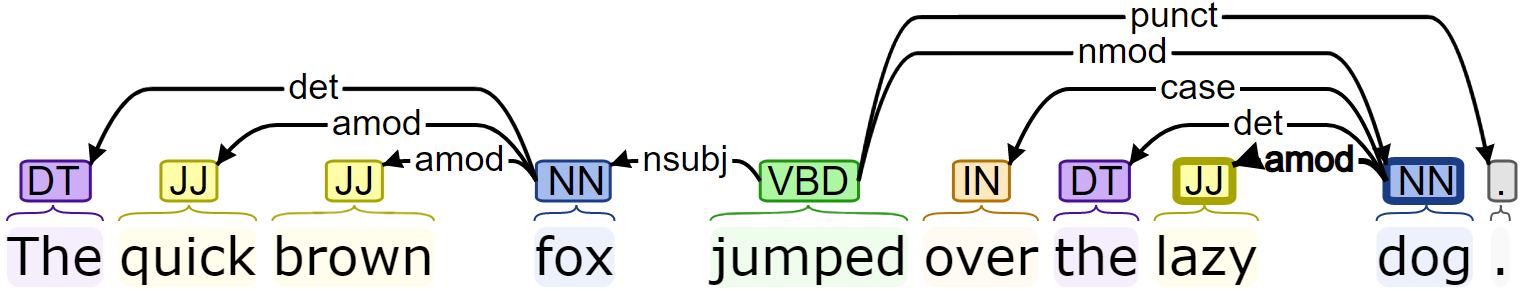
\includegraphics[width=\linewidth]{reports/technical_report/latex/figures/dependency_parse.png}
    \caption{An example of a dependency parse. The arc labelled ``nsubj'' points to the subject of the sentence.
    For a description of what the relations on the arcs mean refer to \citep{martin2018speech}.\protect\footnotemark}
    \label{fig:dependency_parse_example}
\end{figure}

\footnotetext{
    Figure generated from \url{https://corenlp.run/}.
}

\subsection{Edges \& Relating Concepts}
In the graph structure we are building, a relation between concepts is represented as a directed edge between nodes. Edges are used to represent a type of relation where one concept makes reference to, or depends on, another concept. There are three criteria for which I choose to create an edge between two concepts: one concept is the subject of a sentence and the other concept appears in the same sentence; one concept is a noun phrase and the other is a N-bar phrase that is part of the noun phrase; or one concept is a N-bar phrase and the other is a noun that is part of that N-bar phrase. The subject of a sentence can be identified through a dependency parse, which marks the relationships between words in a sentence. See Figure \ref{fig:dependency_parse_example} for an example. 

\begin{figure}
    \centering
    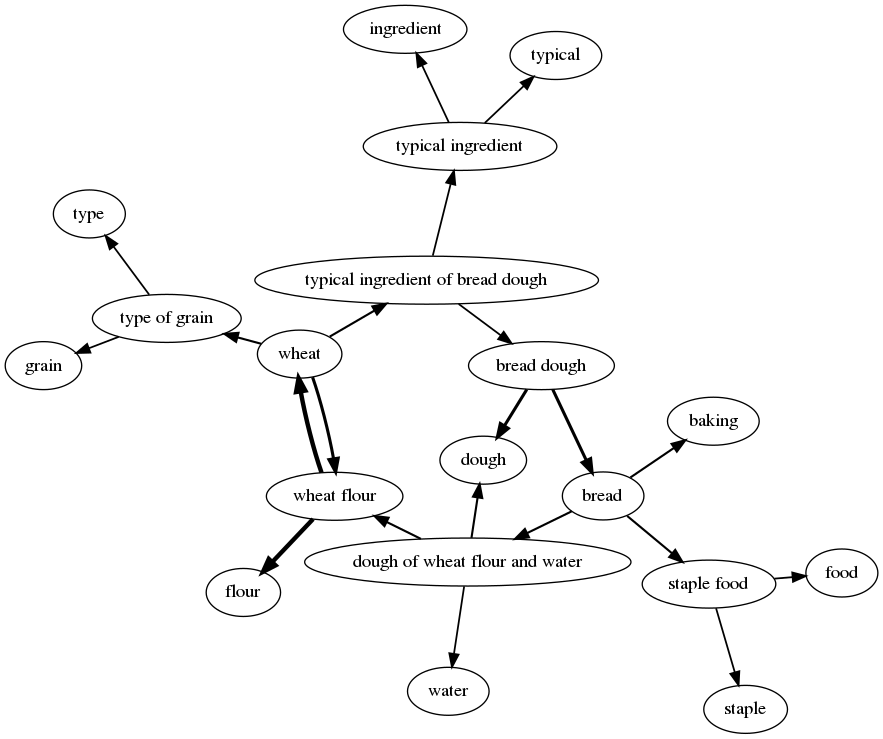
\includegraphics[width=\linewidth]{reports/technical_report/latex/figures/bread_graph-sections_only-implicit_references.png}
    \caption{An example of a dependency-based graph created using the XML document from Figure \ref{fig:sample_xml_document}. Nodes represent the concepts that are referenced in the document. Edges in the graph represent the relationship `A references B'. Blue edges represent forward references and red edges represent backward references.}
    \label{fig:graph_example}
\end{figure}

\subsection{Identifying A Priori \& Emerging Concepts}
A priori and emerging concepts can be identified in a graph by looking at the incoming edges. For a given node, we can look at each of the edges associated with that node. If all of the incoming edges come from nodes in the same section as the node in question, then we can say that the node represents an a priori concept. Otherwise, if there are two or more sections that the incoming edges originate from, then we can say that the node in question represents an emerging concept. 

\subsection{Identifying Forward and Backward References}
In the graph forward and backward references can be found through traversing the graph structure and identifying when the algorithm crosses between sections (see Algorithm \ref{alg:mark edges}). A prerequisite is that we must record the sections that appear in the text, and the order in which they are introduced during the parsing of the text document. We can identify a forward reference when the traversal algorithm visits a node that is associated with a section that comes after the section of the previously visited node. Similarly, backward references can be identified when the traversal algorithm visits a node that is associated with a section that comes before the section of the previously visited node. An example of a graph where the forward and backward egdes have been coloured is shown in Figure \ref{fig:graph_example-coloured_edges}.

\SetKwProg{Fn}{Function}{}{end}
\SetKwFunction{FMarkEdges}{markEdges}
\DontPrintSemicolon

\begin{algorithm*}
    \caption{Marking Forward and Backward References}
    \label{alg:mark edges}
    \KwData{
        $sections$: List of sections in a given document $D$ \\
        $nodes$: Set of nodes in the graph $G$ \\
        $adj$: Adjacency list for a directed graph $G$.\\
    }
    \;
    $visited = \emptyset$\;
    \;
    \For{$node \in$ nodes}{
        markEdges($node$, NULL, visited)\;
    }
    \;
    \Fn{\FMarkEdges{curr, prev, visited}}{
        \tcc{
            Arguments\\
            curr: Current node\\
            prev: Previous node\\
            visited: Set of visited nodes
        }
        \;
        \uIf{$prev \neq NULL$ AND $curr.section \neq prev.section$}{
            $curr\_i \gets sections.indexOf(curr.section)$\;
            $prev\_i \gets sections.indexOf(prev.section)$\;
            \;
            \uIf{$curr\_i < prev\_i$}{
                Mark edge $\{prev, curr\}$ as a backward reference\;
            }
            \uElseIf{$curr\_i > prev\_i$}{
                Mark edge $\{prev, curr\}$ as a forward reference\;
            }
        } 
        \;
        \uIf{$curr \notin visited$}{
            $visited \gets visited \cup \{curr\}$\;
            \;
            \For{neighbour $\in$ adj[curr]}{
                markEdges(\textit{neighbour, curr, visited})\;
            }
        }
    }
\end{algorithm*}

% \subsection{Cycles} 
% We can also consider the number and length of cycles in the graph. Cycles in a graph would suggest the existence of self-referential loops in the text document - in other words sets of concepts that are defined in terms of themselves. Long cycles are perhaps not of too much concern since a long cycle may not necessarily encode a strong dependency between all of the concepts in the cycle. Short cycles, on the other hand may be indicative of strong interdependence and may prove difficult to learn the corresponding concepts since learning one of the concepts in isolation may not suffice.

% \subsection{Isolated and Disjoint Subgraphs} 
% The idea of identifying bottlenecks in the graph structure can be extended to finding subgraphs that form isolated/disjointed clusters. Isolated clusters would be a set of interconnected vertices that have a small number of edges connecting them to the rest of the graph. These clusters would likely represent areas of a knowledge domain that could be learned in relative isolation from the reset of the domain, as long as the bottleneck concepts are learned. Similarly, disjointed subgraphs would also denote a similar thing. The existence of these isolated clusters or disjointed subgraphs would imply lower conceptual density than the alternative - a highly interconnteced graph.

\begin{figure}
    \centering
    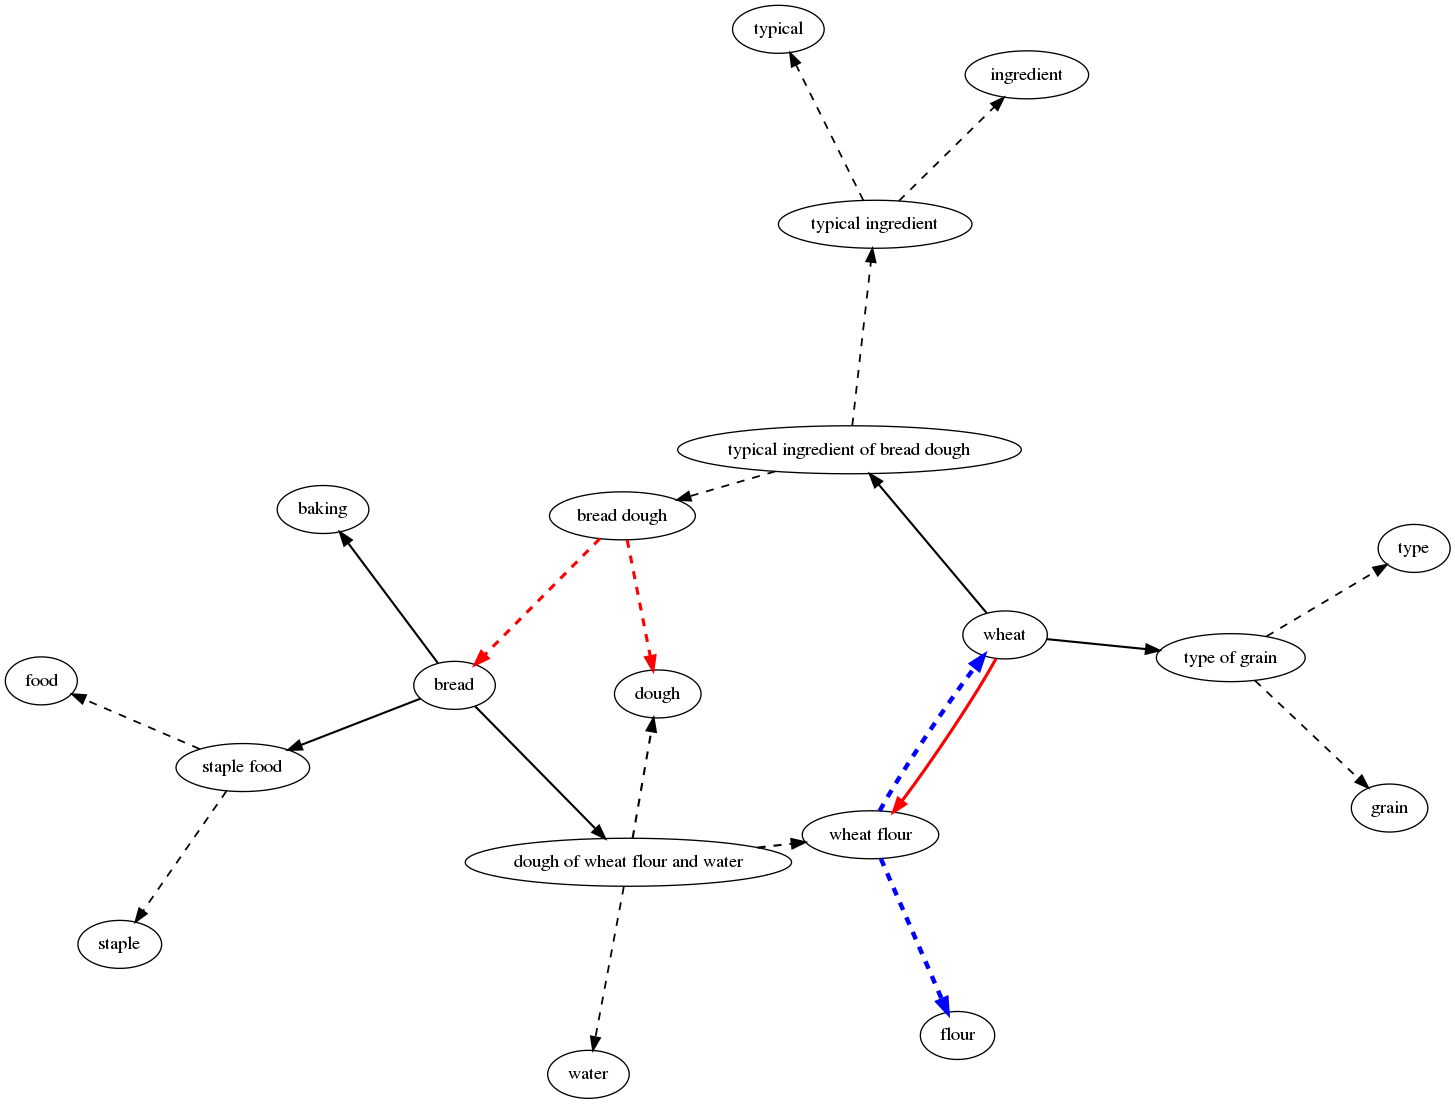
\includegraphics[width=\linewidth]{reports/technical_report/latex/figures/bread_graph-sections_only.png}
    \caption{An example of a dependency-based graph created using the XML document from Figure \ref{fig:sample_xml_document} where forward and backward references have been coloured. Nodes represent the concepts that are referenced in the document. Edges in the graph represent the relationship `A references B'. Blue edges represent forward references and red edges represent backward references.}
    \label{fig:graph_example-coloured_edges}
\end{figure}

\subsection{Deriving a Numerical Score} \label{sec:quantifying_conceptual_density}
At the centre of conceptual density is the notion of the degree to which concepts are integrated. In the graph structure this can be measured by looking at the connectivity of nodes. One useful measure may be the average outdegree:
\begin{equation} \label{eq:simple score}
    S_D = \frac{1}{|V|} \sum_{v \in V} \text{deg}^+(v)
\end{equation}
where $S_D$ is the score of the document $D$, $V$ is the set of vertices in the graph,  and $\text{deg}^+(v)$ is the outdegree, or the number of outgoing edges from the vertex $v$. The interpretation of a high average degree is that the average concept is relatively difficult to learn since the concept is related to many other concepts which you must understand to understand the given concept. 

We can further refine the scoring method by taking into account the strength of the edges, or in other words the weights of the edges:
\begin{equation} \label{eq:weighed score}
    S_D = \frac{1}{|V|} \sum_{v \in V} \sum_{e \in E[v]} e_w
\end{equation}
where $E[v]$ is the set of edges originating from the vertex $v$, and $e_w$ is the weight for a given edge. 
% The previous formulation in Equation \ref{eq:simple score} can be thought of as a special case of this formulation where the weight for every edge is 1.
The weight for given edge can be adjusted based on the type of reference the edge represents. For example, we could set the weight of an edge to: 0.5 for edges that point to a priori concepts since they typically represent a concept that the reader is expected to know beforehand and only impose germane load; 1.5 for backward references to emerging concepts since the reader is required to recall a concept that has been introduced within the text and using a poorly integrated schema will require more mental exertion than when considering an a priori concept; and 2.0 for forward references since the reader is required to \textit{park} a new concept without anything concrete to pin it too, increasing cognitive load. The exact numbers are not important, but rather the relative scales of the numbers. References to a priori concepts should impose less cognitive load than backward references, and backward references should impose less cognitive load than forward references.

\subsection{Summary}
By using part of speech tags and a regex-based chunker we can extract concepts from text. We can then derive relationships between concepts by looking at dependency parses of sentence structures and by looking at the constituent parts of complex concepts represented by noun phrases. For the former method, we simply take the subject of a sentence and create edges between it and each of the other concepts that appear in the same sentence. Concepts are represented as a node in the graph and relationships between concepts are represented as edges in the graph.
The different types of concepts and references can be identified by analysing the edges in the graph. Finally, we can derive a score from the generated graph by measuring the average weighted outdegree.

% Perhaps it is not appropriate to include the number of vertices into the score. After all, the main contributor to conceptual density is not necessarily the number of concepts, but rather the interaction between the concepts and the degree to which the concepts interact. Going back to the element interactivity effect, again we are simply concerned with the number of \textit{interacting} elements. There is bound to be correlation between the number of vertices and the average outdegree, so perhaps information about the number of vertices in the graph is implicitly, and partially, encoded in the measure of average (out)degree. Furthermore, including the number of vertices into the score may lead to bias to longer documents. Longer documents have more opportunities to elaborate and give examples compared to shorter documents. And whether or not a longer document is more conceptually dense than a shorter document should be based on the interactions of the concepts. Thus, I believe that it is best to leave out the number of vertices from the scoring metric, thus reducing the score to:
% \begin{equation} \label{eq:simple score without vertices}
%     S_D = \frac{1}{|V|} \sum_{v \in V} \text{deg}^+(v)
% \end{equation}

% We can further refine the scoring method by taking into account the strength of the edges, or in other words the weights of the edges:
% \begin{equation} \label{eq:weighed score}
%     S_D = \frac{1}{|V|} \sum_{v \in V} \sum_{w \in W_v} w
% \end{equation}
% where $W_v$ is the set of weights for the outgoing edges of the vertex $v$, and $w$ is a single weight for a given edge. The previous formulation in Equation \ref{eq:simple score} can be thought of as a special case of this formulation where the weight for every edge is one.
% The weight for given edge can be adjusted based on the type of reference the edge represents. For example, we could set the weight of an edge to: 0.5 for implicit references since they are not explicitly represented in the text and as such the reader may not need consider the referenced concept; 1.0 for references to a priori concepts since they typically represent a concept that the reader is expected to know beforehand and only impose germane load; 1.5 for backward references since the reader is required to recall a concept that may have been introduced within the text and using a poorly integrated schema will require more mental exertion than when considering an a priori concept; and 2.0 for forward references since the reader is required to \textit{park} a new concept without anything concrete to pin it too, increasing cognitive load. The exact numbers are not important, but rather the relative scales of the numbers. references to a priori concepts should impose less cognitive load than backward references, and backward references should impose less cognitive load than forward references.

% What about references that occur often? If concept A references concept B 100 times, and concept C references concept D 10 times, out of the referenced concepts B and D which would be more difficult to learn? Perhaps a concept being referenced frequently means there are plenty of examples to learn concept B, making it relatively easy to learn concept B. On the other hand, infrequent references to a concept may indicate that the concept is mentioned in passing or as an example and that the concept is relatively simple. Maybe just looking at the frequency of references does not give us enough information to decide this. In this report I will use the interpretation that highly frequent references indicate a higher level of interdependence between two concepts, and as such higher conceptual density. I choose to incorporate frequency into the score by taking a weighted frequency:
% \begin{equation} \label{eq:weighed frequency score}
%     S_D = \frac{1}{|V|} \sum_{\{x, y\} \in E} w(x, y) f(x, y)
% \end{equation}
% where $E$ is the set of all edges $\{x, y\} $ in the graph, $w: \{x, y\} \mapsto \mathbb{R}^+$ is a function that maps the edge $\{x, y\}$ to a weight, and $f: \{x, y\} \mapsto \mathbb{Z}^+$ is a function that maps the edge $\{x, y\}$ to a frequency count.

% One possible issue with Equation \ref{eq:weighed frequency score} is that a reference with a frequency of 40 is not necessarily much more important than a reference with a frequency of 20. In extreme cases, how important is the frequency of a reference when we get to frequency counts of  100 and 200. There is a point where a higher frequency does not really mean much. Thus, it may be sensible to scale down large frequency counts. I do this by scaling the weighted frequency logarithmically: \todo{what is the precedent for this? (Zipf's law, typical language models, tf-idf?)}
% \begin{equation} \label{eq:log weighed frequency score}
%     S_D = \frac{1}{|V|} \sum_{\{x, y\} \in E} 1 + \text{log}_2 (1 + w(x, y) f(x, y))
% \end{equation}
% where I add one to the argument to the log function so that the most basic reference (weight of one, frequency of one) results in zero, in other words no effect. Adding one to the logarithmically-scaled weighted frequency means that the minimum contribution of an edge to the score is one.

% However, as discussed in Section \ref{sec:presentation of concepts} not all references are created equal. So the type of reference should be taken into account. This is done by assigning different weights to the different types of references. We can also include the frequency of references (e.g. how often A references B) and combine it with the associated weights. I also scale this weighted frequency logarithmically in case a single or few concepts are dominant in a text. For example, in this paper words such `concept' and `graph' appear in almost every section and mentioned frequently. These types of dominant concepts may skew the score of an otherwise simple document and so I scale the frequency count of references.

% Including cycles and disjointed subgraphs, we can define a scoring scheme of conceptual density for a given document as such:
% \begin{equation*}
% 	\begin{aligned}	
%     S_D =\ &|C| + \frac{1}{|C|} \sum_{c \in C} |c| \\ 
%     			&+ |M| + \frac{1}{|M|} \sum_{m \in M} |m| \\
%     			&+  \frac{1}{|V|} \sum_{\{x, y\} \in E} 1 + \text{log}_2 (1 + w(x, y) f(x, y))
% 	\end{aligned}
% \end{equation*}
% where $S_D$ is the score for a given text document $D$, $C$ is the set of simple cycles in the graph, $c$ is a simple cycle in $C$, $M$ is the set of disjointed subgraphs in the graph, $m$ is a disjointed subgraph in $M$, $V$ is the set of all vertices (nodes) in the graph, $E$ is the set of all edges $\{x, y\} $ in the graph, $w: \{x, y\} \mapsto \mathbb{R}^+$ is a function that maps the edge $\{x, y\}$ to a weight, and $f: \{x, y\} \mapsto \mathbb{Z}^+$ is a function that maps the edge $\{x, y\}$ to a frequency count.
%  I add one to the argument to the log function so that the most basic reference (weight of one, frequency of one) results in zero, in other words no effect. Adding one to the log term means that the minimum contribution of an edge to the score is one.

\section{Related Work} \label{sec:related_work}
\subsection{Information Extraction}
The process of identifying concepts and how they are related that I have described in this report is similar to the task of information extraction. However, there are some key differences between what I have done and what is usually done in information extraction. First and foremost, information extraction is typically concerned with named-entity recognition - the identification of named-entities such as names of people, companies, locations, and dates. In this project we are concerned with concepts in general (all types of entities), which can be thought of as a superset of named-entities. Furthermore, information extraction is also interested in the relationship between named-entities. However, in this project and the work-to-date we are not too concerned about the nature of a relationship between concepts as much as the fact that a relationship exists.

\begin{figure}
    \centering
    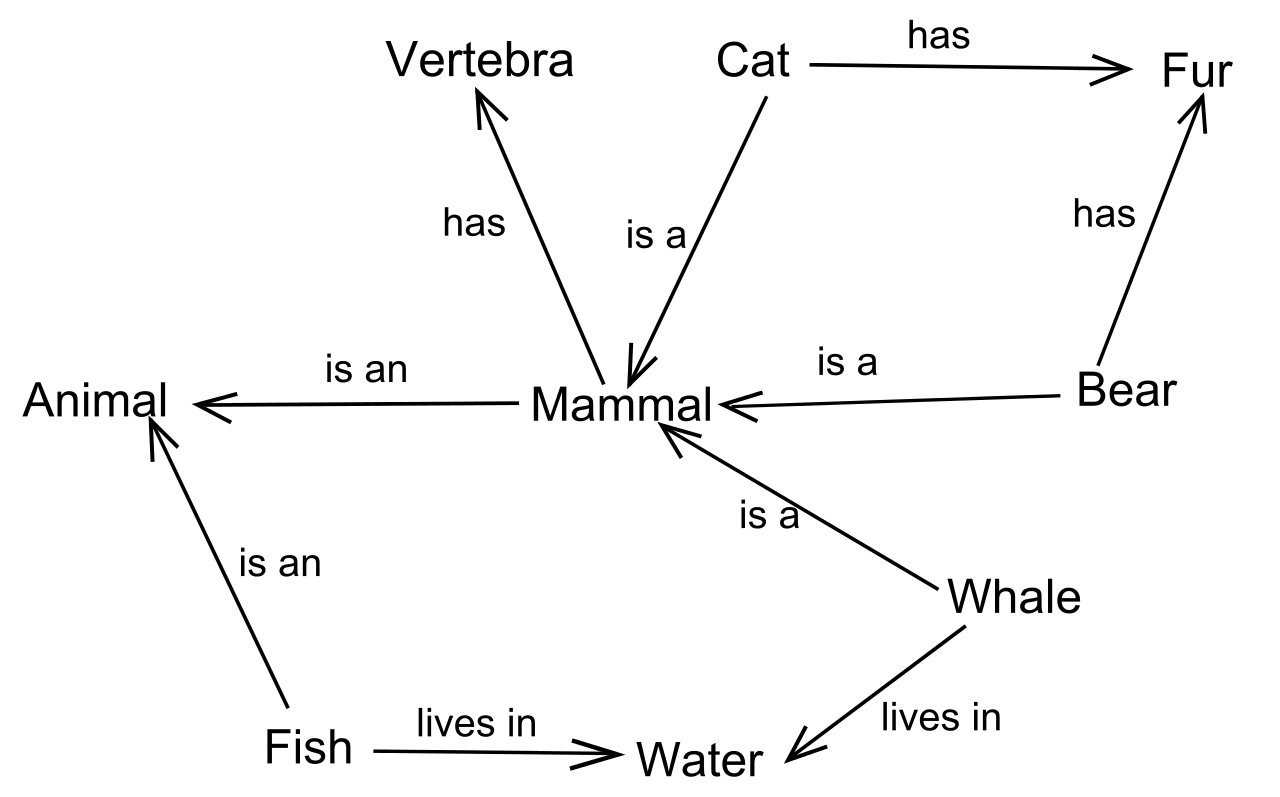
\includegraphics[width=\linewidth]{reports/technical_report/latex/figures/semantic_map_example.png}
    \caption{An example of a semantic network.\protect\footnotemark}
    \label{fig:semantic_network_example}
\end{figure}

\footnotetext{Figure from \url{https://commons.wikimedia.org/wiki/File:Semantic_Net.svg}.}

\subsection{Semantic Networks \& Knowledge Graphs}
The type of graph structure that is being built up in this project is very similar to semantic networks/knowledge graphs. Some differences between the graphs in this project and semantic networks are that: we are not annotating edges with the type of relationship (compare Figure \ref{fig:graph_example-coloured_edges} and Figure \ref{fig:semantic_network_example}, for example), and the criteria for deciding what constitutes a node or edge in the graph may differ from what is common in the literature. For one, somewhat complex noun phrases are added as nodes in this project rather than just the head of a noun phrase.

% \subsection{Automatic Generation of Mind Maps from Text}
% In \citep{abdeen2009direct} a tool for automatically generating mind maps from text was proposed. This has many similarities to this project in the way that a graph structure is being built from a text document. However like information extraction and semantic networks, this mind map tool is focused on extracting concepts and assigning distinct relationships between concepts. At present, in this project we are more interested in just the existence of a relationship. Further more, the tool does not support

\section{Future Work} \label{sec:future_work}
\subsection{Transitioning to Unstructured Text}
In the current implementation a graph can be built from semi-structured text (e.g. Figure \ref{fig:graph_example}), but recreating the same graph from the corresponding plain text version of a document remains difficult. At present the sections and section headers must be explicitly marked up in XML. Moving to unstructured text is desirable since using semi-structured text requires someone to manually mark up the text, which is a time consuming process. Identifying the section titles and where sections start and end can be unreliable at times when using regex pattern matching due to different section heading formats and it is liable to false positives (see Table \ref{tab:section_finding_example} in the appendix, for example). 

\subsection{Improving Information Extraction}
One issue with the current work is the quality of the extracted concepts and how the concepts are related. There are many cases where the extracted concepts do not align with the concepts or relations that a human would intuitively pick out. While the current quality is adequate enough to build up a graph structure, important concepts and relations between concepts are likely to be missed. So it is important that future work focuses on improving the quality of extracted concepts and relations. Improving the current implementation would include extending the definition of a concept in text to include verbs and verb phrases, and another thing to improve would be the quality of the extracted relations between concepts. 

However, there exists a framework called OpenIE \citep{banko2007open} which is made for performing information extraction, which is essentially the task that I am trying to perform. The benefits of using such a framework is that many of the issues with the current implementation for extracting concepts and relations between concepts in this project have more or less been solved in OpenIE. One issue with using OpenIE in this project is that it generates many spurious tuples (see Table \ref{tab:openie_example} in the appendix for an illustrative example). So if OpenIE were to be used in this project the main thing that would need to be worked on is filtering the triples.

% \subsubsection{Extending the Definition of a Concept in Text}
% In addition to noun phrases we can include other types of phrases into the definition of a `concept'. We can extend the definition of noun phrases to include two noun phrases joined by a preposition. For example, consider the phrase ``relationships between concepts''. Under the previous definition we would consider ``relationships'' and ``concepts'' as two separate noun phrases, however it is equally sensible to consider the entire phrase as a single entity. We can also include particular types of verb phrases. For example, consider the sentence ``Listening to music is his favourite way to pass time'', what are the concepts being talked about here? I believe it would be sensible to say that the concepts of ``listening to music'' and ``passing time'' are being discussed. Adding these types of phrases leads to a more rich definition of a `concept'. 

% \subsubsection{Better Dependency Parsing}
% The current scheme for relating concepts in the dependency-based graph simply relates the subject of a sentence to the other concepts that appear in the sentence. This does not capture the nuances of natural language very well. For example, consider the sentence ``Wheat is used for making wheat flour, a typical ingredient of bread dough'' from Figure \ref{fig:sample_txt_document}. Under the current scheme the subject, `Wheat', would have an edge created between itself and the other concepts `wheat flour' and `typical ingredient of bread dough'. However, the sentence is phrased such that wheat flour is being to referred to as a `typical ingredient of bread dough', not `wheat'. A more correct set of edges in this case would connect `wheat' to `wheat flour' and `wheat flour' to `typical ingredient of bread dough'. 

% \subsubsection{Information Extraction Frameworks} Much of the work in this project has been inspired by other work but built from scratch. As discussed earlier, much of the process of extracting and relating concepts is similar to the task of information extraction. There exists a framework called OpenIE \citep{banko2007open} which is made for performing information extraction. The benefits of using such a framework is that many of the issues with the current dependency parsing in this project have more or less been solved in OpenIE. An issue with using OpenIE in this project is that it generates many spurious tuples (see Table \ref{tab:openie_example} in the appendix for an illustrative example). So if OpenIE were to be used in this project the main thing that would need to be worked on is filtering the triples.
% Perhaps there are patterns in the dependency parse that could be used to assign the correct relation in this sort of case.
%In this particular case, `wheat flour' is the direct object of `making' and `typical ingredient` is the appositive modifier of `wheat flour'.

\subsection{Additional Graph Features}
There are many graph analysis techniques that have not been explored in this report. For example, see \citep{algorithms_documentation}. It would be interesting to see if incorporating features derived from these analysis techniques into the scoring scheme would improve it. For example, we could look at: identifying simple cycles in the graph using Johnson's algorithm; identifying minimum cuts which could be used to identify bottleneck concepts and to find subgraphs that are \textit{isolated} in the sense that they are mostly separate from the main supergraph; and reachability of nodes in the graph.

% \subsubsection{Bottlenecks} \label{sec:bottlenecks}
% Another interesting possible feature in the graph topology is the idea of a bottleneck vertex/vertices that might be able to be found by identifying the minimum cuts of the graph. One could imagine a bottleneck in a graph structure being visually similar to a hourglass.
% % (see Figure \ref{fig:bottleneck example} in  \ref{sec:supplementary figures} for an example).
% The vertex at the centre of the hourglass shape would be the bottleneck vertex. This would correspond to a concept that is defined in terms of other concepts and is used to define a set of other concepts. For example, in programming polymorphism and inheritance cannot be explained if classes are not explained, similarly classes cannot be explained if variables and functions are not explained. While in this example we could imagine back references from polymorphism to functions, to explain polymorphism we must first explain classes. Therefore, directionality must included when defining and identifying bottleneck concepts. Bottleneck concepts are important to the idea of conceptual density because they make learning more difficult.

% \subsubsection{A priori concepts}
% It may be possible to redefine what an a priori concept is in terms of sinks in a graph. A sink is a node in a directed graph that has an outdegree of zero, i.e. it has no outgoing edges. Identifying sinks in a graph is trivial, but we could also extend the idea of an a priori concept being a concept that is only referenced from within one section to: a concept that only leads to a sink and is not part of a self-referential system. \todo{Can also identify emerging concepts by looking sentences where the subject is followed by `is a'}

\subsection{Additional Text Features}
There are other features that could be extracted from text.
In \citep{robins2010learning} it is suggested that a measure of distance between keywords (concepts) could be used to help measure conceptual density and included in the scoring scheme. There are some methods that may help with this such as: using lexical chains for keyword extraction \citep{ercan2007using}; and looking at long distance dependency as a metric of reading comprehension difficulty \citep{liu2008dependency}. 

\subsection{Evaluation of the Model} \label{sec:evaluation_of_the_model}
Regarding the evaluation of the model for quantifying conceptual density, the quality of the scores have not been evaluated. Since no objective measure of conceptual density exists in the current literature, there exists no benchmarks to compare the model with. The next best thing to compare the model against is human judgements. One experiment that could be done is to gather a collection of snippets from textbooks. These snippets would consist of a few chapters from a given textbook. Then we could arrange the collection into pairs and get human judgements on whether or not the first snippet is more conceptually dense than the second snippet. From there, for each document pair we could generate scores using the model described in this report and determine which document the model judges as being more conceptually dense. Then we could compare the model's judgements to the human judgements to evaluate how `good' the model is, or how well it follows human intuition.

% One particular experiment that I envision is one performed on a labelled data set of abstracts created from human judgements. We need to use human judgements since, as discussed near the start of this report, there no objective measures of conceptual density or element interactivity and as such human judgements are the only baseline available to compare the model with. For the collection of documents, we could gather a number of snippets from various textbooks that consist of a few sections. The reason for choosing snippets that contain is that they are short, self-contained, expository documents. And if we are to get human judgements then it will be a lot easier and a lot less time consuming to use abstracts as apposed to long documents such as textbooks. Once a collection of abstracts have been created we could group abstracts into pairs and get a panel of human judges to judge which document appears to be more conceptually dense.  Then, we could compare the output of the model against the human judgements and see how well it mimics the human judgements.

% \subsection{Feature Importance Analysis}
% From the process described in Section \ref{sec:evaluation_of_the_model} we would create a labelled data set. From this we could train a machine learning algorithm such as a simple linear regression or random forest. Then through feature importance analysis we could investigate which features out of all of the extracted features (from text and the graph structure) are the most salient in regards to conceptual density. And with a large enough data set, we could simply extract as many features as possible, regardless of whether or not they seem relevant to conceptual density, and then use this feature importance analysis to filter out the unimportant features in a principled way. It should be noted that this is likely outside the scope of the project.

\section{Conclusion} \label{sec:conclusion}
In this report I have explored a graph-based approach to quantifying conceptual density - an idea relating to the degree that concepts of a particular knowledge domain, encoded by a text document, are integrated. I have discussed how this idea of conceptual density is grounded in, and related to, learning edge momentum and cognitive load theory. I have discussed the ways in which the notion of conceptual density can be defined and measured in semi-structured and unstructured text documents. By analysing the language in the documents and observing the patterns in natural language we can create an operational definition of a `concept' in text. Then by analysing the relationships between concepts in a given document we can build up a graph structure from which we can derive a score of conceptual density. 


% \bibliographystyle{acm}
\bibliography{report}


% % Activate the appendix
% % from now on sections are numerated with capital letters
% \appendix

% % \renewcommand{\thesection}{Appendix \Alph{section}}

% \section{Implementation Details}
% \begin{itemize}
%     \item Parsing Unstructured Text
    
%     \begin{itemize}
%         \item Normalisation Techniques
%         \item Sentence and Word Tokenisation
%         \item POS Tagging
%         \item Regex Chunking
%         \item Constituency Trees
%     \end{itemize}
% \end{itemize}

% \subsection{Relevant NLP Methods?}
% \begin{itemize}
%     \item Parts of Speech Tagging
%     \item Constituency Parsing/Chunking
%     \item Dependency Parsing
% \end{itemize}

% \subsection{Relevant Graph Analysis Techniques?}
% \begin{itemize}
%     \item Minimum cut
% \end{itemize}

% % \section{Synthesised Text Corpus}
% % We created a small corpus of hand-crafted text documents. These can be separated into three main groups: one group where the text is as simple as possible and is minimally conceptually dense; one group where ideas are dependent on the ones preceding it; and one final group where an attempt was made to make the most entangled mess possible. The idea is that each of these groups of texts will have characteristics that we believe will lead to low, medium, and high conceptual density respectively, purposefully inserted.

% \section{Supplementary Figures} \label{sec:supplementary figures}

% \begin{sidewaysfigure}
%     \centering
%     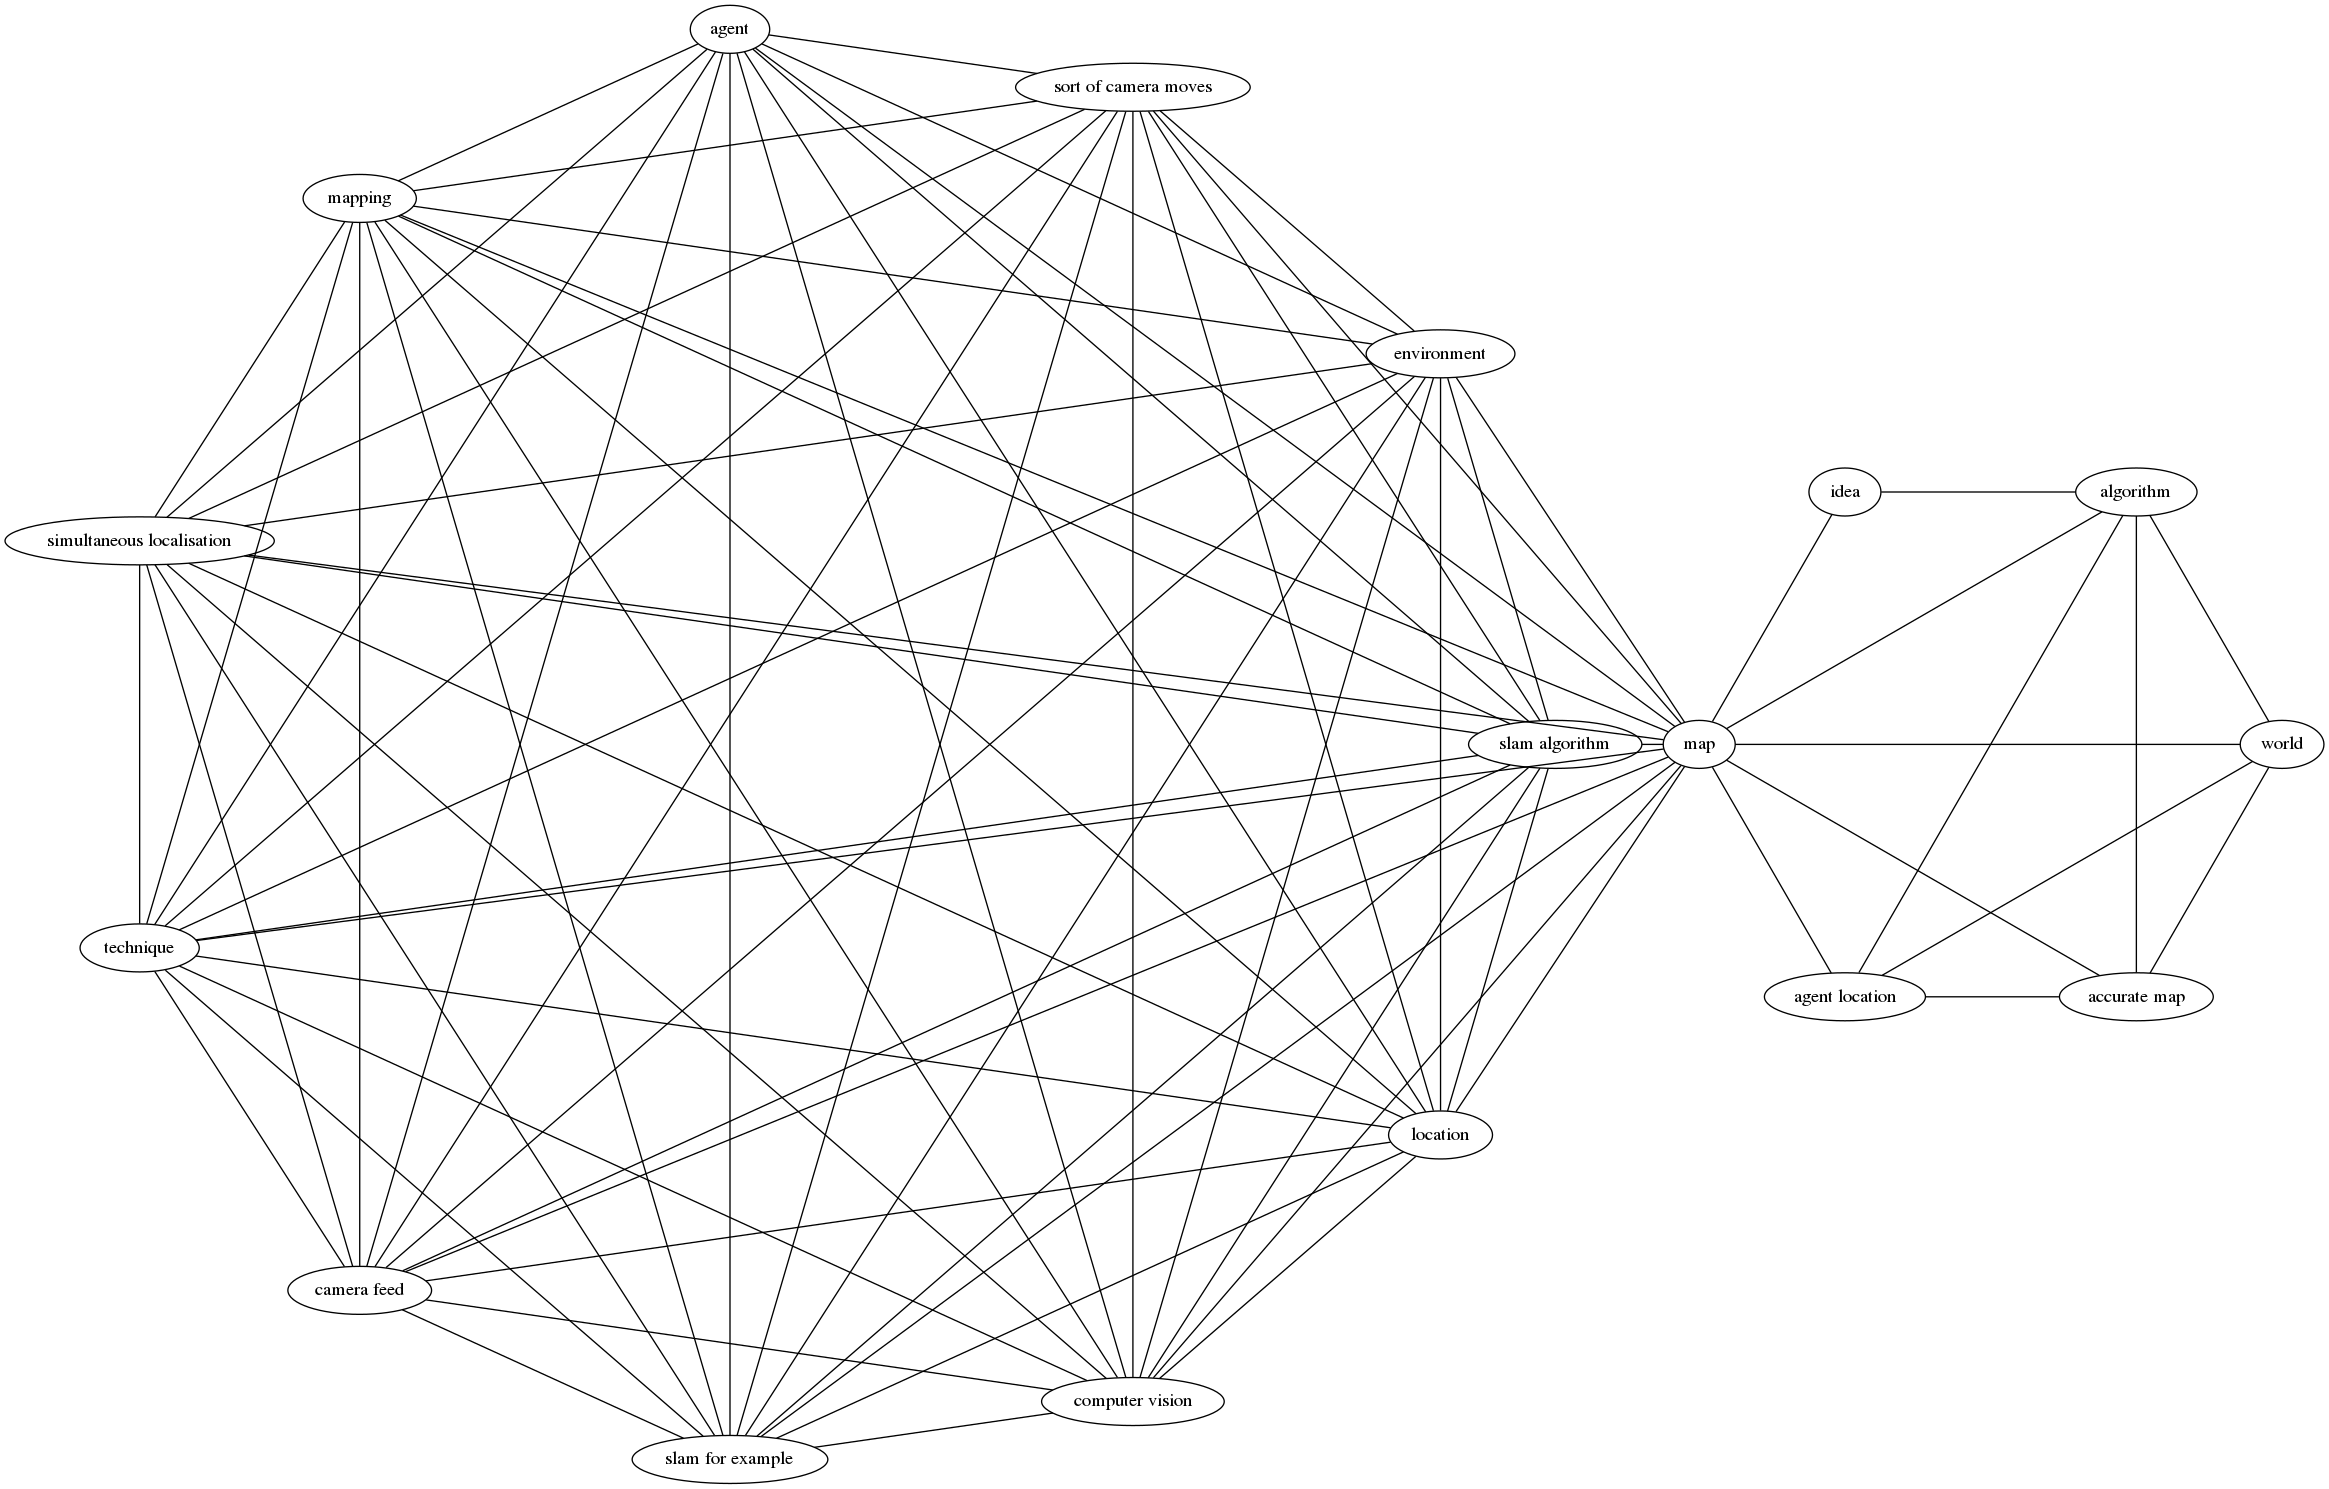
\includegraphics[width=\linewidth]{reports/technical_report/latex/figures/bottleneck.png}
%     \caption{An example of a graph built from unstructured text using simple co-occurrence. Notice that the graph is densely connected, and that it also forms the sort of hourglass structure mentioned in Section \ref{sec:bottlenecks}}
%     \label{fig:bottleneck example}
% \end{sidewaysfigure}

\appendix
\section{Tables}
\begin{longtable}{|p{8cm}|r|r|}
    \caption{An example of the current implementation for finding section headers, start and end positions generated from  \citep{sweller2011element}.}
    \label{tab:section_finding_example} \\
    \hline
    \textbf{Section Header} & \textbf{Start Pos.} & \textbf{End Pos.} \\
    \hline
    \endfirsthead
    
    \hline
    \textbf{Section Header} & \textbf{Start Pos.} & \textbf{End Pos.} \\
    \hline
    \endhead
    
    Chapter 15 & & \\
    The Element Interactivity Effect &  44 & 3358 \\ 
    \hline
    Empirical Evidence for the Element Interactivity Effect &  3359 & 8850 \\ \hline
    *\textit{The secondary task was presented on a separate computer and involved a tone} &  8851 & 9091 \\ 
    \hline
    *\textit{When instructional materials involved low or no interaction between elements} of &  9092 & 9964 \\ 
    \hline
    Element Interactivity and Understanding Instructions &  9965 & 10041 \\ 
    \hline
    *\textit{The extent to which we understand instructions depends on levels of element} &  10042 & 12129 \\ 
    \hline
    Element Interactivity and the Modality Effect &  12130 & 16477 \\ 
    \hline
    Element Interactivity and the Expertise Reversal Effect &  16478 & 18835 \\ \hline
    Element Interactivity and the Imagination Effect &  18836 & 21474 \\ 
    \hline
    Conditions of Applicability &  21475 & 21908 \\ 
    \hline
    *\textit{There is also an obvious relation between these two effects as the levels of element
    interactivity that produce an intrinsic cognitive load are always relative to levels of} &  21909 & 24226 \\ 
    \hline
    Instructional Implications &  24227 & 26005 \\ 
    \hline
    Conclusion &  26006 & 27782 \\ 
    \hline
\end{longtable}

\begin{longtable}{|l|l|p{8cm}|} 
    \caption{An example of the relation triples extracted from the document in Figure \ref{fig:sample_txt_document} illustrating how OpenIE generates many spurious triples. Notice that some entities in the column `Entity 2' are nonsensical, e.g. ``staple food by usually baking''.} 
    \label{tab:openie_example} \\
    \hline
    \textbf{Entity 1} & \textbf{Relation} & \textbf{Entity 2} \\
    \hline
    \endfirsthead
    
    \hline
    \textbf{Entity 1} & \textbf{Relation} & \textbf{Entity 2} \\
    \hline
    \endhead
    Bread    &	is	&    food typically prepared from dough by baking \\
    \hline
    Bread    &	is	&    staple food prepared \\
    \hline
    Bread    &	is	&    staple food typically prepared from dough of wheat flour usually by baking \\
    \hline
    Bread    &	is	&    food typically prepared from dough \\
    \hline
    Bread    &	is &    food by	baking \\
    \hline
    Bread    &	is	&    staple food typically prepared from dough usually by baking \\
    \hline
    Bread    &	is	&    staple food prepared from dough by baking \\
    \hline
    Bread    &	is	&    food typically prepared usually by baking \\
    \hline
    Bread    &	is	&    food prepared \\
    \hline
    Bread    &	is	&    food typically prepared \\
    \hline
    Bread    &	is	&    staple \\
    \hline
    Bread    &	is	&    food prepared from dough of wheat flour by baking \\
    \hline
    Bread    &	is	&    staple food typically prepared \\
    \hline
    Bread    &	is &    staple food by	baking \\
    \hline
    Bread    &	is	&    food prepared from dough by baking \\
    \hline
    Bread    &	is	&    staple food typically prepared by baking \\
    \hline
    Bread    &	is	&    staple food prepared from dough of wheat flour by baking \\
    \hline
    Bread    &	is	&    food typically prepared from dough of wheat flour \\
    \hline
    Bread    &	is	&    staple food \\
    \hline
    Bread    &	is	&    food typically prepared by baking \\
    \hline
    Bread    &	is	&    staple food typically prepared from dough of wheat flour by baking \\
    \hline
    Bread    &	is	&    food typically prepared from dough of wheat flour by baking \\
    \hline
    Bread    &	is	&    staple food typically prepared from dough \\
    \hline
    Bread    &	is	&    food prepared from dough \\
    \hline
    Bread    &	is	&    food prepared from dough of wheat flour \\
    \hline
    Bread    &	is	&    staple food typically prepared usually by baking \\
    \hline
    Bread    &	is	&    staple food prepared from dough usually by baking \\
    \hline
    Bread    &	is	&    staple food prepared from dough of wheat flour usually by baking \\
    \hline
    Bread    &	is &    food by	usually baking \\
    \hline
    Bread    &	is	&    food prepared usually by baking \\
    \hline
    Bread    &	is	&    food prepared by baking \\
    \hline
    Bread    &	is &    staple food by	usually baking \\
    \hline
    Bread    &	is	&    food typically prepared from dough of wheat flour usually by baking \\
    \hline
    Bread    &	is	&    food prepared from dough usually by baking \\
    \hline
    Bread    &	is	&    staple food prepared usually by baking \\
    \hline
    Bread    &	is	&    staple food prepared by baking \\
    \hline
    Bread    &	is	&    staple food typically prepared from dough by baking \\
    \hline
    Bread    &	is	&    staple food typically prepared from dough of wheat flour \\
    \hline
    Bread    &	is	&    staple food prepared from dough of wheat flour \\
    \hline
    Bread    &	is	&    food \\
    \hline
    Bread    &	is	&    food typically prepared from dough usually by baking \\
    \hline
    Bread    &	is	&    food prepared from dough of wheat flour usually by baking \\
    \hline
    Bread    &	is	&    staple food prepared from dough \\
    \hline
    Wheat    &	making	&    ingredient of bread dough \\
    \hline
    Wheat    &	making	&    wheat flour \\
    \hline
    Wheat    &	making	&    ingredient \\
    \hline
    Wheat    &	is	&    commonly used \\
    \hline
    wheat flour    &	ingredient of	&    bread dough \\
    \hline
    Wheat    &	making	&    typical ingredient of bread dough \\
    \hline
    Wheat    &	making	&    typical ingredient \\
    \hline
    Wheat    &	is	&    used \\
    \hline
\end{longtable}

\end{document}